%\figureRight{4cm}{handy}
\section{Informationsquellen}

\subsection{Lernplattform Moodle}
Die wichtigste Quelle für Lernstoff ist, neben der Vorlesung, das Lernportal Moodle. Zu finden unter \url{www.moodle.hm.edu}.
Die Anmeldung erfolgt mit dem Hochschul-Account (E-Mail ohne "@hm.edu")\doublebreak
In Moodle stellen euch viele Professoren die Vorlesungsunterlagen zur Verfügung. Oftmals müssen Abgaben dort hochgeladen und kleine Tests, die den Stoff abfragen, gemacht werden.
In der ersten Vorlesung geben euch die Professoren meist das Passwort zu dem jeweiligen Moodle-Kurs der Lehrveranstaltung, damit nur Studierende die auch in die Vorlesung gehen, die Unterlagen bekommen.

\subsection{Schwarzes Brett}
Die wichtigste Quelle, um z.B. zu erfahren, wann man sich wo im ZPA einschreiben kann, ob eine Vorlesung/ein Praktikum ausfällt, etc. ist das Schwarze Brett.\doublebreak 
Am besten abonniert ihr das Schwarze Brett direkt als Feed in euren RSS Reader: \url{feed://fi.cs.hm.edu/fi/rest/public/news.rss} oder per Mail über \url{www.cs.hm.edu/meinstudium/studierenden\_services/fi\_studierendenlogin.de.html}.\\
Informationen wie Ausfälle, Abgabetermine, Zuordnungen für Wiederholer und vieles mehr werden hier bekannt gegeben.
Auf der Website der Fachschaft \url{fs.cs.hm.edu} und in der FachschaftsApp haben wir für euch eine \red{sortierte und gefilterte Ausgabe} des Schwarzen Bretts
programmiert. Damit lassen sich für euch relevante Informationen noch schneller finden.

\subsection{Aushänge}
Im 3.Stock findet ihr in den Schaukästen vor dem Sekretariat viele 
aktuelle Informationen zu eurem Studium. Hier wird auch als Erstes im 
Semester der \red{Stundenplan} ausgehängt. In den
Schaukästen vor den Professorenbüros könnt ihr oft \red{Stellenanzeigen} 
für das Praxissemester oder \red{Themen für Abschlussarbeiten} finden. 
Weitere Stellenanzeigen und Jobangebote findet ihr auch im 
Erdgeschoss im Gang vor der Fachschaft. 

\subsection{FS-Website und FS-App}
\begin{itemize}
	\item Die Homepage der Fachschaft findet ihr unter \url{https://fs.cs.hm.edu}.
	\item Unsere \red{FachschaftsApp} für Android findet ihr im Playstore. 
	Einfach nach „FK07“ suchen.
	\item Unsere \red{FachschaftsApp} für iOS ist derzeit noch in Arbeit.
\end{itemize}

\subsubsection{Raumsuche}
Ihr müsst noch eine Abgabe fertig machen oder wollt mit Kommilitonen 
lernen und braucht einen Raum dafür? Auf unserer Fachschafts-Website unter
\begin{sitenav}
	\item \url{https://fs.cs.hm.edu}
	\item TOOLS
	\item Raumsuche
\end{sitenav} oder in der
\red{FachschaftsApp} könnt ihr nach freien Räumen suchen.

\subsubsection{FS-News}
Auf der Fachschafts-Website \url{https://fs.cs.hm.edu} tragen wir, unter der Kategorie FS-News, alle Themen zusammen die euch interessieren könnten, wie z.B. 
aktuelle Veranstaltungen, Partys, Projekte und Wissenswertes sowohl 
von uns als auch überfakultär. 

\subsection{FI-Services}
Die FI-Services sind alle wichtigen Informationen gesammelt auf einer 
übersichtlichen Seite ohne Schnickschnack. Hier findet ihr vor allem 
schnell die Stunden- und Prüfungspläne der Fakultät 07 und vieles mehr.
\url{www.fi.cs.hm.edu}\doublebreak
Die Stundenpläne für die BWL-Fächer für Wirtschaftsinformatik 
findet ihr auf 
\begin{sitenav}
	\item \url{www.bwl.hm.edu}
	\item VORLESUNGSPLAN
\end{sitenav}
und natürlich in unserer FSApp.
Ein Besuch lohnt sich auf jeden Fall!

\subsection{Sekretariat}
Neben der Fachschaft können euch auch unsere äußerst engagierten 
Damen im Sekretariat bei allen Belangen eures Studiums weiterhelfen. 
Das Sekretariat befindet sich im dritten Stock etwa in der Mitte der 
linken Gebäudeseite.\doublebreak
Hier nur ein paar Punkte bei denen das Sekretariat weiter hilft:
\begin{itemize}
	\item \red{Labor/Hörsaal zu gesperrt?} 
	\item Wenn ihr bei der Scheinausgabe nicht da wart, landen die \red{Scheine im Sekretariat}	
	\item \red{Abgabe von Praktikumsberichten/-Zeugnissen} (in Kopie) (werden an das Prüfungsamt weitergeleitet) 
	\item Abgabe von Anmeldung und Abschlussarbeit 
	\item Verträge für Tutoren/Studentische Hilfskräfte 
	\item Pflege vom Schwarzen Brett und Aushängen 
	\item Wenn die Professoren nicht zur Vorlesung kommen
	\item Anlaufstation für Verlorengegangenes
\end{itemize}
Die aktuellen Öffnungszeiten findet ihr auf der Homepage der Fakultät. 

\subsection{Infopoint}
Der Infopoint ist Anlaufpunkt für allgemeine Fragen bezüglich des 
Studiums. Ihr findet ihn im Haupteingang in der Lothstraße 34 auf der 
rechten Seite. Telefon: \red{(089) 12 65 - 0}\\
\begin{center}
	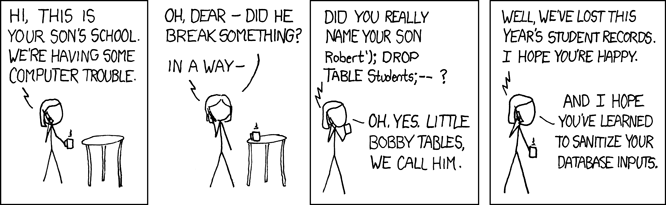
\includegraphics[width=12cm]{inputs/Bilder/name_of_son.png}
\end{center}
